\documentclass{llncs}

\usepackage[utf8]{inputenc}
\usepackage{hyperref}
\usepackage{times}
\usepackage[T1]{fontenc}
\usepackage{listings}
\usepackage{graphics}
\usepackage{graphicx}
\usepackage{multicol}
\usepackage[a4paper, top=3.5cm, bottom=2cm, left=2cm, right=2cm]{geometry}
\usepackage{float}

\lstset{language=C, frame=tlrb, basicstyle=\scriptsize, breaklines=true, numberbychapter=false,numbers=left}

\begin{document}

\bibliographystyle{splncs}

\title{Lessons learned from contrasting a BLAS kernel implementations}
\author{Andrés More\inst{1} \inst{2}}

\institute{Intel Software Argentina (Argentina Software Design Center) \\
\email{andres.more@intel.com} \\ 
\and
Instituto Aeronáutico Córdoba \\
\email{amore@iua.edu.ar}}

\maketitle

\begin{abstract}
This work reviews the experience of implementing different versions of the SSPR rank-one update operation
of the BLAS library. The main objective was to contrast CPU versus GPU implementation effort and complexity of an optimized BLAS routine, not considering performance. 
This work contributes with a sample procedure to compare BLAS kernel implementations,
how to start using GPU libraries and offloading, how to analyze their performance and
the issues faced and how they were solved.

\keywords{BLAS libraries, SSPR kernel, CPU architecture, GPU architecture, Performance analysis, Performance measurement, Software Optimization.}

XIII Workshop de Procesamiento Distribuido y Paralelo
\end{abstract}

\section{Introduction}

With the growth of the application of general-purpose GPU techniques to compute intensive problems \cite{gpgpu}, there will be lots of domain experts trying to implement an specific math kernel operation both in CPU and GPU, applying optimizations and finally doing a performance comparison to double check if gains are relevant due the invested effort \cite{gpuorg}.

\smallskip

It is non trivial to identify the outcome. While CPUs are designed for general purpose, GPUs are designed for specific purposes;  specific problems are well suited to GPU architecture and can be solved faster than using CPUs, but they
usually need to be represented in a way parallelism is explicitly exposed.
Picking the right approach will contribute to faster, more detailed problem solving in domain specific problems.
It is expected that the procedure of reviewing an specific kernel implementations will be done on each release of new CPU and GPU architecture by people doing problem solving simulations. From that point of view this work contributes with a similar analysis experience. Related work is included as part of the results as a validation proof.

\smallskip

The rest of the document is structured as follows: this section is completed with information on the operation and system being used for the comparison, plus a quick discussion on the GPU programming model. Section 2 include details on which algorithms were executed after reviewing well-known implementations. Section 3 provide details on how the performance was contrasted, including results and related work validating our results.

\subsection{Single-precision Symmetric Packed Rank-one update}

The Single-precision Symmetric Packed Rank-one update (SSPR) operation computes a rank-1 update of a symmetric matrix of single precision floating point numbers. SSPR performs the symmetric rank 1 operation show in Equation \ref{eq:math},
where $ \alpha $ is a real scalar, $ x $ is an $ n $ element vector and $ A $ is an
$ n $ by $ n $ symmetric matrix, supplied in packed form.

\begin{equation}
    A := \alpha \times x \times x ^{T} + A
\label{eq:math}
\end{equation}

A graphical representation of the operation is shown in Figure \ref{fig:math}.

\begin{figure}[H]
\begin{center}
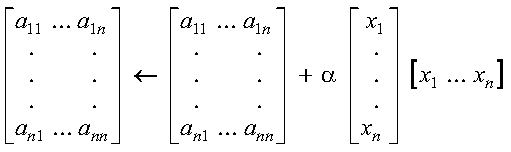
\includegraphics[scale=0.7]{math.png}
\caption{Graphical representation of rank 1-update}
\label{fig:math}
\end{center}
\end{figure}

The SSPR operation belongs to level 2 BLAS (Basic Linear Algebra Subprograms) \cite{blas} \cite{blas-updated},
as it runs over a matrix-vector combination. Matrix-vector multiplication has $ O(N^{2}) $ complexity on the size of the matrix \cite{matmul}.  However, the matrix is required to be represented as a vector which contains only half of the symmetric matrix triangular, packed sequentially per column. Represented by Equation \ref{eq:packed}. In particular, the vector has a size of $ (n \times (n + 1) / 2) $. This approach avoids redundancy and saves device memory for bigger input.

\begin{equation}
AP(i + ( j \times (j-1) / 2) = A _{ij} (\forall j \geq i)
\label{eq:packed}
\end{equation}

Operation signature in the Fortran language is defined in Listing \ref{lst:signature} and clarified in Table \ref{table:args} below. Towards generality of the function, UPLO specifies if the packed triangular matrix is the upper or the lower part of the original data. INCX is the required increment to reference the vector elements in the provided vector reference. This is useful to iterate over a vector which is part of a matrix, avoiding extra buffer copies.

\begin{lstlisting}[language=FORTRAN, caption={SSPR Fortran Signature}, label={lst:signature}]
SUBROUTINE SSPR(UPLO, N, ALPHA, X, INCX, AP)
          .. Scalar Arguments ..
          REAL ALPHA
          INTEGER INCX,N
          CHARACTER UPLO
          ..
          .. Array Arguments ..
          REAL AP(*),X(*)
\end{lstlisting}

\begin{table}
\caption{SSPR Arguments Description}
\centering
\begin{tabular} {|l|l|} \hline
{\bf Argument} & {\bf Description} \\ \hline
UPLO & Specifies whereas upper/lower triangular part of A is supplied in array \\ \hline
N & Specifies the order of the matrix A \\ \hline
ALPHA & Specifies the scalar alpha \\ \hline
X & Array of dimension at least $ ( 1 + ( n - 1 ) * abs( INCX ) ) $ \\ \hline
INCX & Specifies the increment for the elements of X \\ \hline
AP & Array of dimension at least $ ( ( n*( n + 1 ) ) / 2 ) $ \\ \hline
\end{tabular}
\label{table:args}
\end{table}

\subsection{Testbed}

The system used for experiments was an {\it HP Mobile Workstation EliteBook 8530w}, having integrated
an {\it Intel CPU model T9600} \footnote{\href{http://ark.intel.com/products/35563}{T9600 CPU specifications}}
plus a {\it Quadro FX 770m GPU} \footnote{\href{http://www.nvidia.com/docs/IO/57883/PO\_Quadro\_FAM\_Mar08\_FINAL\_LowRes.pdf}{Quadro FX 770m GPU specifications}}. Although the system is a little bit outdated and it is not state-of-the-art, the computing devices were integrated at the same time-frame and hence provide a valid point of comparison.

\smallskip

The relevant information from their hardware specifications are shown below. The CPU information was taken from {\tt /proc/cpuinfo} and a custom program to access GPU attributes not yet exposed thru standard kernel interfaces.

\begin{verbatim}
cpu family: 6
model: 23
model name: Intel(R) Core(TM) 2 Duo CPU T9600 @ 2.80GHz
stepping: 10
cpu MHz: 2793
cache size: 6144 KB
fpu: yes
cpuid level: 13
flags: fpu vme de pse tsc msr pae mce cx8 apic sep mtrr
pge mca cmov pat pse36 clflush dts acpi mmx fxsr sse sse2
ss ht tm pbe pni dtes64 monitor ds_cpl vmx smx est tm2
ssse3 cx16 xtpr pdcm sse4_1 xsave osxsave lahf_lm
TLB size: 0 4K pages
\end{verbatim}

The GPU card has built-in 512MB memory, meaning that in average during executions
there is about 462 MB of global memory available for computation.

\begin{verbatim}
capabilities.name = Quadro FX 770M
capabilities.totalGlobalMem = 512.00 MB
capabilities.sharedMemPerBlock = 16.00 KB
capabilities.regsPerBlock = 8192
capabilities.warpSize = 32
capabilities.memPitch = 2097152.00 KB
capabilities.maxThreadsPerBlock = 512
capabilities.maxThreadsDim = 512 512 64
capabilities.maxGridSize = 65535 65535 1
capabilities.totalConstMem = 64.00 KB
capabilities.major = 1
capabilities.minor = 1
capabilities.clockRate = 1220.70 MHz
capabilities.textureAlignment = 256
capabilities.deviceOverlap = 1
capabilities.multiProcessorCount = 4
cudaMemGetInfo.free = 462 MB
\end{verbatim}

As depicted in Figure \ref{fig:flops}, the different in single-precision (real) floating point operations is significant.
It might be expected results that choose GPUs as the winner, which will be a different assumption if the operation was using double precision floating point operations.

\begin{figure}[H]
\begin{center}
\begin{tabular}{cc}
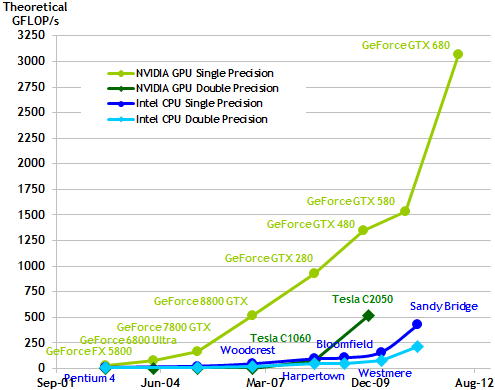
\includegraphics[scale=0.46]{flops.png} & 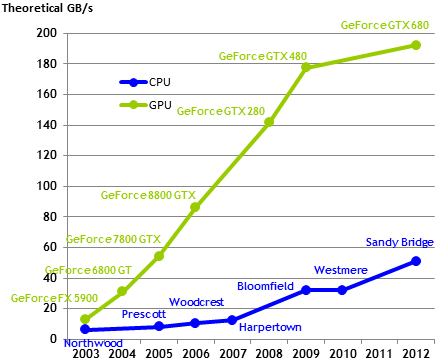
\includegraphics[scale=0.5]{bw.png} \\
\end{tabular}
\caption{FLOPs and Bandwidth Comparison between CPUs and GPUs \cite{cuda}}
\label{fig:flops}
\end{center}
\end{figure}

\subsection{CUDA Programming}

The Compute Unified Device Architecture (CUDA) is a high performance computing architecture and programming
model created by NVIDIA. The CUDA programming model gives access to GPUs instruction
set to be used for general purpose computing, providing both low level and high level interfaces to simplify
application.

\smallskip

The programming model assumes that the host system will execute kernels by asynchronous offloading
to a GPU device. Memory allocation and transfer are also controlled by the developer. The programming
model relies on a hierarchy of thread groups that can access per-group shared memory and can synchronize
between them. An extension to the C language allows the inclusion of compute kernels that run in the GPU
device. Hardware threads are part of an N-dimensional block with {\tt N=1,2,3}.

\smallskip

All threads on a block are expected to share (faster than global) memory resources and to synchronize
with each other. Blocks per-se are also organized in sets called grids, similar to blocks. Thread blocks
perform independent computation. Each block memory hierarchy consists of local, global, shared, constant
and texture memory; the latter having special addressing to better fit graphical rendering. All but shared
memory is persistent across kernel executions.

\smallskip

GPU hardware and software capabilities are evolving fast, not only instructions per cycle have increased.
Support for native arithmetic instructions have expanded the set of atomic operations and the provided math
functions. The usual {\tt printf} capability has been recently made available, the runtime uses a special device
buffer that it is transferred together with the device memory. It is worth noting that IEEE 754-2008
binary floating-point arithmetic has deviations from standard by default. Enabling strict support imposes
a performance penalty.

\section{Algorithms}

As part of the work 4 different versions of SSPR functions were exercised, using well-known implementations as a reference. 
The following subsections contains details on how the versions were implemented that can be reused for any other BLAS kernel. In order to streamline analysis only support for upper matrices with 1 increments were incorporated.

\subsection{CPU Sequential}

Using both the original BLAS implementation \footnote{\href{http://www.netlib.org/blas/sspr.f}{BLAS SSPR implementation.}} and the GNU Scientific Library version \footnote{\href{gsl/blas/source\_spr.h}{GSL SSPR implementation.}} an initial CPU sequential version was implemented as shown in Listing \ref{lst:naive}.
It is worth to note that any BLAS kernel can be reviewed also on this two implementations.
A naive implementation of the mathematical definition was not used as proper speedup computation requires best known sequential algorithm \cite{debunking}, shown in Listing \ref{lst:cpuopt}.

\begin{lstlisting}[caption={Naive SSPR CPU Implementation},label={lst:naive}]
k=0;
for (j=0;j<n;j++)
	for(i=0;i<=j;i++) {
		ap[k] += alpha*x[i]*x[j];
		k++;
}
\end{lstlisting}

\begin{lstlisting}[caption={Optimized SSPR CPU Implementation},label={lst:cpuopt}]
for (i = 0; i < n; i++) {
	const float tmp = alpha * x[i];

	for (j = 0; j <= i; j++)
		ap[((i * (i+1)) / 2+j )] += x[j] * tmp;
}
\end{lstlisting}

Here it can be estimated that the required computation per data quantity is not enough to justify accelerator offload time. It is expected then that a GPU version of it is not going to have huge performance increments for small data.

\subsection{GPU cuBLAS}

This implementation was done directly reusing CUDA source code.
NVIDIA CUDA \cite{cuda} provides its own version of BLAS routines, which are heavily optimized to their architecture. Using the {\it cuBLAS} \cite{cublas} library requires one call, an example is shown in Listing \ref{lst:gpucublas}.

\begin{lstlisting}[caption={cuBLAS SSPR GPU Implementation}, label={lst:gpucublas}]
ret = cublasSspr(handle, mode, n, &alpha, cx, incx, cap);
if (ret != CUBLAS_STATUS_SUCCESS)
	err("cublasSspr: %d (%s)", ret, cublas2str[ret]);
\end{lstlisting}

This highly optimized code can be found in the package available to registered developers,
inside {\tt sspr.cu} and {\tt sspr.h} files. The main routine is {\tt cublasSspr()}. 
This implementation first loads into device shared memory elements reused during computation, then computes several matrix elements for hardware thread. It also uses cheap left bit-shifting instructions instead of expensive division-by-2 to locate elements inside the packed matrix.

\smallskip

The library documentation recommends the use of on utilities like: {\tt cublasCreate()}, {\tt cublasSetVector()},
{\tt cublasGetVector()}, {\tt cublasDestroy()}. They provide easier allocation of memory on the GPU device.
The library also defines opaque data-types for parameters and error handling such as: {\tt cudaError\_t},
{\tt cublasHandle\_t}, {\tt cublasStatus\_t}, {\tt cublasFillMode\_t}.

\subsection{GPU Naive}

A naive GPU implementation is useful to have a worst-estimate to be compared against potential optimizations.
A direct translation to GPU using one thread per vector element to computing the result in parallel is shown in Listing \ref{lst:gpunaive}. Here it is assumed that the number of elements in $ x $ it is close to the number of GPU threads.

\begin{lstlisting}[caption={Naive SSPR GPU Implementation},label={lst:gpunaive}]
__global__ void sspr_naive_kernel(int uplo, int n, float alpha, const float *x, int incx, float *ap) {
	int i = blockIdx.x * blockDim.x + threadIdx.x;
	if (i < n) {
		const float tmp = alpha * x[i];
		int j = 0;
		for (j = 0; j <= i; j++)
			ap[((i*(i+1))/ 2 + j)] += x[j] * tmp;
	}
}
\end{lstlisting}

How to execute the kernel is shown in Listing \ref{lst:gpukernel}. CUDA will run a preprocessor transforming the code before performing actual compilation.

\begin{lstlisting}[caption={GPU Kernel execution},label={lst:gpukernel}]
int threads = capabilities.maxThreadsPerBlock;
sspr_naive_kernel <<< (n / threads), (threads) >>> (uplo, n, alpha, cx, incx, cap);
\end{lstlisting}

\subsection{GPU using shared-memory}

The recommended approach to start optimizing GPU code is to use shared memory to reduce access time to data.
Every thread on the same thread block loads in shared memory one element of the vector, this work is done in parallel and a barrier is used to synchronize. During computation, elements are then gathered from faster shared memory when possible, slower global memory is used otherwise. The implementation is shown in Listing \ref{lst:gpuoptimized}.

\begin{lstlisting}[caption={Optimized SSPR GPU Implementation},label={lst:gpuoptimized}]
__global__ void sspr_optimized_kernel(int uplo, int n, float alpha, const float *x, int incx, float *ap) {
	int i = blockIdx.x * blockDim.x + threadIdx.x;
	if (i < n) {
		int tid = threadIdx.x;
		extern __shared__ float cache[];
		float *xi = (float *) cache;
		xi[tid] = x[i];
		__syncthreads();
		const float tmp = alpha * x[i];
		int j = 0;
		for (j = 0; j <= i; j++) {
			if (blockIdx.x * blockDim.x < j &&	blockIdx.x * blockDim.x + 1 > j)
				ap[((i*(i+1))/ 2 + j)] += xi[j] * tmp;
			else
				ap[((i*(i+1))/ 2 + j)] += x[j] * tmp;
		}
	}
}
\end{lstlisting}

However, this method does not take into account any other potential optimization, it is included here to show that naive optimizations are not preferred and it is more useful to build upon CUDA implementation source code.

\section{Performance Analysis}

This section includes details on how the performance of the different implementations were conducted. The tools and procedure can be reused for any other BLAS kernel without major modifications.

\subsection{GPU Registers}

The CUDA {\tt nvcc} compiler can be configured to show extra information about the number of registers used during execution. With this option the code can be optimized so register usage metric is minimal.

\begin{verbatim}
ptxas info: Compiling entry function 'sspr_naive' for 'sm_13'
ptxas info: Used 7 registers, 48+16 bytes smem, 4 bytes cmem[1]
ptxas info: Compiling entry function 'sspr_optimized' for 'sm_13'
ptxas info: Used 10 registers, 48+16 bytes smem, 4 bytes cmem[1]
\end{verbatim}

It was discovered that running with the {\tt --arch=compute\_11} option did not included this output,
but using {\tt --arch=sm\_13} instead solved the issue. The first one uses the compute capability version to specify the hardware target, while the second uses the hardware architecture generation.

\subsection{Nvidia Visual Profiler}

The {\tt nvvp} tool depicts a visual execution profile of the program, useful when trying to understand where the computation is spending execution time. On our case, even with {\it cuBLAS} implementation the tool identified:

\begin{itemize}
\item there is no overlap between data transfer and computation
\item the data transfer action does not fully saturate available memory bandwidth
\item the computation does not fully load processing cores capacity
\end{itemize}

The affected GPU device does not have enough internal memory to run an interesting enough problem,
the required computation per transfered bytes does not justify GPU offloading.

\begin{figure}[H]
\begin{center}
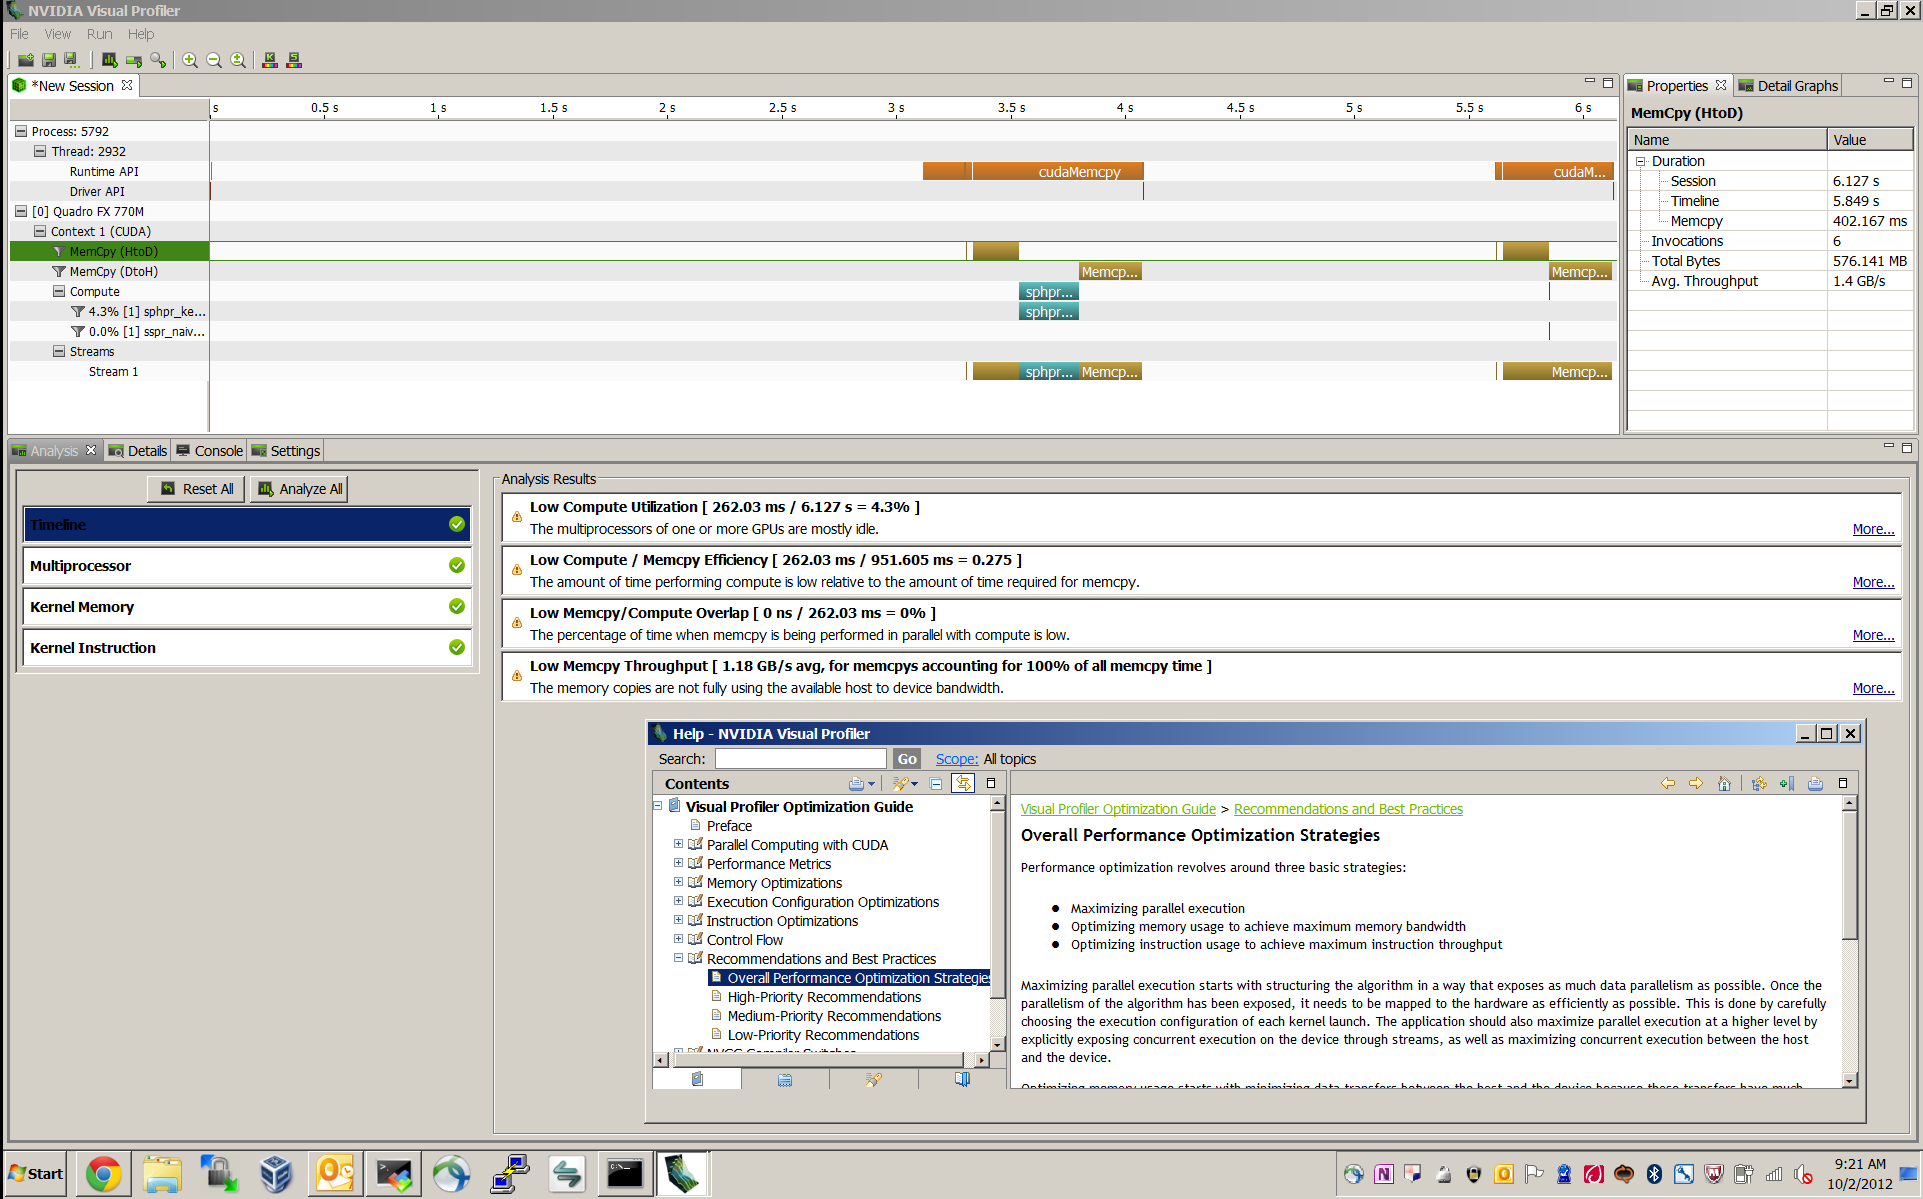
\includegraphics[scale=0.25]{profiler.png}
\caption{GPU Profiler}
\label{fig:profiler}
\end{center}
\end{figure}

\subsection{Results}

Figure \ref{fig:speedup} shows wall clock times in seconds with varying matrix sizes.
\footnote{Times are the geometric mean of 32 executions in order to reduce measurement noise.
To validate results the output matrix was reduced to a single figure being the common global sum of the elements.}
Here it can be seen that the CPU optimized version is taking the least time on all of the matrix sizes.
On the other hand we double check that the GPU naive and shared-memory optimized versions are not a match against the CUDA one provided by cuBLAS. Here it can be clearly confirmed that the introduced shared memory optimization do not positively impact execution time, so {\it cuBLAS} strategy is hence superior. 

\begin{figure}[H]
\begin{center}
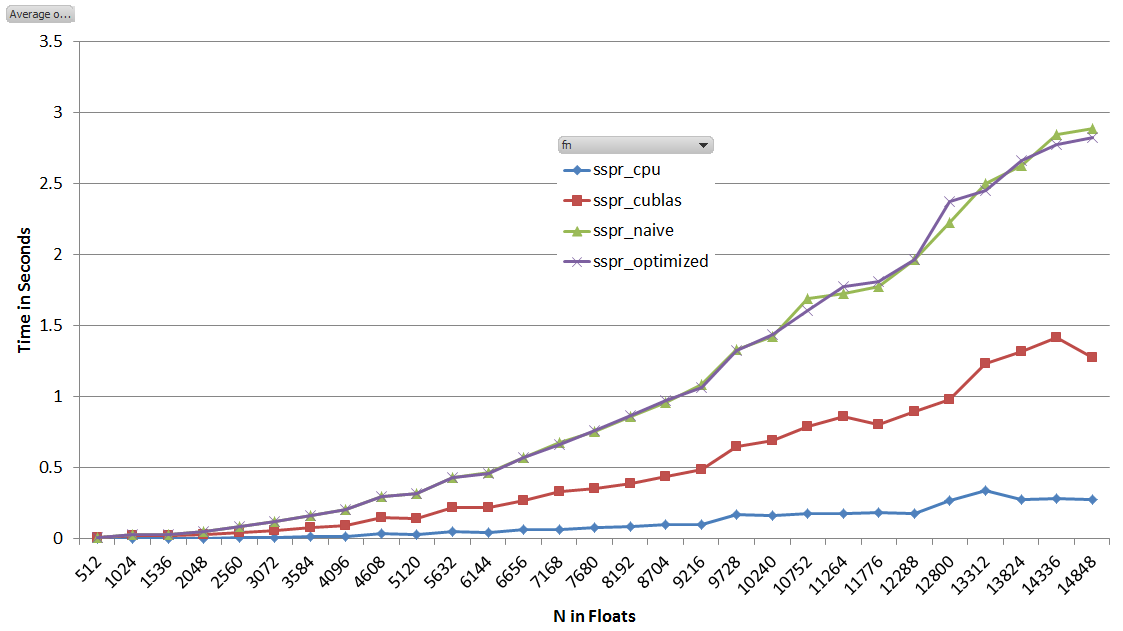
\includegraphics[scale=0.4]{speedup.png}
\caption{Execution Time Speedup}
\label{fig:speedup}
\end{center}
\end{figure}

\subsection{Speedups}

To measure speedups the input size was selected as big as possible to fit inside the available memory in GPU. This is always recommended to maximize computation per transfered byte. The time taken to transfer the data to the GPU is included on the measurements, the goal was to contrast the complete operation execution from start to end.

\begin{verbatim}
SSPR_N = 14848 floats (packed 110238976 floats)
SSPR_ALPHA = 3.141593
memory = 420 MB
cudaMemGetInfo.free = 462 MB
\end{verbatim}

Most interesting speedup comparisons are shown in Table \ref{table:speedup}. The optimized CPU version has nearly 4x of cuBLAS version, and close to 8x of our naive implementations using GPU. It is interesting to note that cuBLAS optimization got 2x speedup when matched against our naive optimization with shared memory.

\begin{table}
\caption{Speedup comparisons}
\centering
\begin{tabular} {|l|l|l|} \hline
cublas (1.4995 seg) & cpu (0.389625 seg) & 3.85x \\ \hline
naive (3.090625 seg) & cpu (0.389625 seg) & 7.93x \\ \hline
optimized (2.97325 seg) & cpu (0.389625 seg) & 7.63x \\ \hline
naive (3.090625 seg) & cublas (1.4995 seg) & 2.06x \\ \hline
optimized (2.97325 seg) & cublas (1.4995 seg) & 1.98x \\ \hline
optimized (2.97325 seg) & naive (3.090625 seg) & 0.95x \\ \hline
\end{tabular}
\label{table:speedup}
\end{table}

\subsection{Related Work}

There is a related study conducted by Microsoft Research \cite{ms-gaxpy}, that performed benchmarking of BLAS Level
2 routines in FPGA, CPU and GPU. Their findings in Figure \ref{fig:gaxpy} validates the results obtained as part of this work. An an optimized implementation in CPU is better than an optimized GPU implementation. Note that {\it Intel Math Kernel} library version is still far better than an optimized CPU version, as it uses advanced knowledge of the architecture of computing units inside the CPU.

\smallskip

It is worth to note that state-of-the-art GPU devices have increased their internal memory to cope with this limitation, up to 4GB in latest 2012 boards. If ECC is enabled to verify contents then this quantity is decreased 10\%. A detailed analysis on how to better exploit GPU performance is reviewed in \cite{similar} using a complete application as case study.

\begin{figure}[H]
\begin{center}
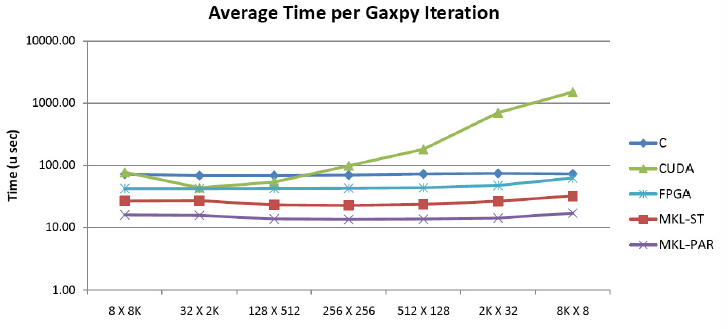
\includegraphics[width=12cm]{gaxpy.png}
\caption{Independent measurement of matrix-vector kernels (extract from \cite{ms-gaxpy})}
\label{fig:gaxpy}
\end{center}
\end{figure}

\section{Conclusions}

This works provides a sample procedure to contrast BLAS kernel implementations after a experience with the SSPR operation. Source code pointers details are provided that guides through well-known implementation, also include performance analysis tools and their application example. In order to gather performance figures, it is always recommended to review the optimized code of BLAS instead of doing naive implementations. It is also worth to note that efficient GPU offload requires significant amounts of required computation per transfered byte. In this case, matrix-vector kernel computation showed that CPUs provide better results than GPUs; even when using highly optimized implementations of the kernel operation.

\smallskip

Regarding the experience with CUDA, the cuBLAS library documentation and interface properly support
development, although they can still be improved. Some utility calls like {\tt cublasAlloc()} are deprecated
but still referenced by {\tt cudaSspr()} and others, confusing the reader. The library does not provide a wrapper
call that goes over the complete offload cycle: initialization, data transference to and from accelerator,
explicit computation, etc. Using the documented primitives plus required error checking implies nearly 60
lines of code, just to offload one BLAS routine. cuBLAS also lacks an error formatter function to translate error
codes to text representations (similar to {\tt strerr()}). If it is required to support both Linux and Windows
environments, the usual time keeping routines are not portable so a {\tt gettimeofday()} stub was coded that
could have been provided by the CUDA runtime instead.

\smallskip

Regarding further work, developing a framework to quickly benchmark compute kernels on different processing devices will be of value to domain experts researching what type of hardware to acquire. Ideally, including support for state-of-the-art BLAS implementations to provide figures from optimized algorithms. Also extending the comparison will be a good initial step, including other parallel programming techniques and technologies like OpenMP and MPI. Including results from other devices like FPGAs and co-processors would be another interesting option. There are other GPU optimizations that although require advanced knowledge (i.e. overlapping communication and computation, using texture memories) may result in better performance figures. Upcoming GPU architectures having more memory or new hardware-assisted features
(i.e. zero-copy data replication) may also show different results.

% \section*{Acknowledgments}

% The author would like to recognize the help from colleges at the Argentina Software Design Center, and the reviewers for the quality feedback they have provided.

\bibliography{sspr}

\end{document}
